\documentclass[12pt]{article}
\usepackage[top=3cm,bottom=2cm,left=3cm,right=2cm]{geometry}
\usepackage[utf8]{inputenc}
\usepackage[english,brazil]{babel}
\usepackage{graphicx}
\usepackage{float}



\begin{document}
	
	\title{\textbf{Uso de jogos digitais no ensino}}
	\author{\textit{Denilson Sousa}\\\textit{Ismael Moreira}}
	
	\maketitle % Data

	\selectlanguage{brazil}
	\begin{abstract}
		Este artigo tem como objetivo mostrar a eficiência do uso de jogos digitais no ensino. Para ele desenvolvemos um jogo chamado \textit{Run Aedes} que tem como objetivo informar sobre o \textit{Aedes Aegypti}. Aplicamos o jogo em uma escola da nossa cidade e colhemos alguns dados importantes e curiosos sobre o comportamento das pessoas (jovens) no uso do software.
	
		\textbf{Palavras-chave}: Jogos Educativos; Aedes Aegypti; Jogos Digitais;  Jogos no ensino.	
	\end{abstract}


	\selectlanguage{english}
	\begin{abstract}
		This article aims to show the efficiency of the use of digital games in teaching. For him we developed a game called \textit {Run Aedes} that aims to inform about \textit {Aedes Aegypti}. We apply the game to a school in our city and we collect some important and curious data about the behavior of people (young people) in the use of the software. \\
			
		\textbf{Palavras-chave}: Educational games; Aedes Aegypti; Digital games; Games in education.	
	\end{abstract}
	
	
			
			
	\section{Introducao}%Na introdução, deve-se apresentar o tema do artigo e a problemática em que se insere. %Também se deve apresentar como a pesquisa foi realizada para discussão do item-problema.
	
	Da Antiguidade até o início do século XIX, predomina na prática-escolar uma aprendizagem de tipo passivo e receptivo. Aprender era quase exclusivamente memorizar. Neste tipo de aprendizagem, a compreensão desempenhava um papel muito reduzido(Eulina Castro de Souza, Ilana Castro de Souz, Vany Regina Teixeira).\\
	
	Os conhecimentos a serem adquiridos eram, até certo ponto, reduzidos. E para que os alunos pudessem repetí-los correta e adequadamente, o professor utilizava o procedimento de perguntas e respostas, tanto em sua forma oral como escrita. Este era o chamado método catequético, cuja origem remota, pelo menos cultura ocidental, aos antigos gregos. A palavra catecismo provém do termo grego katechein, que significa "fazer eco". Este método era usado por todas as disciplinas e consistia na apresentação, pelo professor, de perguntas acompanhadas de suas respostas já prontas.(Eulina Castro de Souza, Ilana Castro de Souz, Vany Regina Teixeira)\\
	
	Ao ensinar um assunto o professor deve:\\
	
	Apresentar o objeto ou idéia diretamente, fazendo demonstração, pois o aluno aprende através dos sentidos, principalmente vendo e tocando.\\
	
	Mostrar a utilidade específica do conhecimento transmitido e a sua aplicação na vida diária.
	Fazer referência à natureza e origem dos fenômenos estudados, isto é, às suas causas.\\
	
	Explicar primeiramente os princípios gerais e só depois os detalhes.\\
	
	Passar para o assunto ou tópico seguinte do conteúdo apenas quando o aluno tiver compreendido o anterior.(Eulina Castro de Souza, Ilana Castro de Souz, Vany Regina Teixeira)\\
	
	Com o decorrer do tempo esses métodos de ensino se tornam cada vez mais cansativos no olhar dos alunos. Com a tecnologia avançando e as pessoas cada vez mais imersas nesse mundo a forma de ensino não pode ficar parada no tempo, a tecnologia veio para nos auxiliar em tarefas consideradas difíceis isso inclui o ensino. Há um tempo atras as pessoas já vinham com ideias de melhorar o ensino com o uso de jogos, jogos educativos como: Blocos de montar, Quebra-cabeça, jogos de tabuleiro… todos tem como um objetivo a diversão, porém, estimulam o raciocínio logico desde crianças até adultos, por isso a importância de continuar investindo em jogos como uma forma de ensinar não só o raciocínio logico, mas como qualquer área, desde matérias escolares até tópicos mais abstratos como comunidade, social, prevenções, etc...
	
	Este artigo esta dividido em 4 partes (incluindo a introdução), na primeira parte temos uma breve introdução sobre a problemática que estamos apresentando e dando algumas alternativas de solução, na segunda parte está os métodos utilizados, onde explicamos qual método utilizamos para propor nossas ideias e o por que escolhemos essa técnica, na terceira parte vamos falar sobre a pesquisa, como a pesquisa foi elaborada, aplicada e analisada, na quarta parte terá nossa conclusão onde vamos repassar todos os conhecimentos e dados colhidos nessa pesquisa.
	
		
		
	\section{Método utilizado}% Qual método nois utilizamos para fazer essa pesquisa, no nosso caso foi uma %pesquisa aplicada
	Nosso Objetivo nesse artigo é demostrar a eficiência do uso de jogos para o ensino seja ele qual for. Desse modo tivemos que ter algo que nos possibilitasse mostrar essa eficiência, por isso desenvolvemos o jogo \textbf{Run Aedes} para que pudéssemos aplicar o mesmo e colher as informações necessárias. Nesse âmbito utilizamos o método de pesquisa aplicada, com questionários, que poderia nos fornecer uma pesquisa eficiente e rápida.
	
	A pesquisa aplicada tem como objetivo a utilização de toda informação disponível para a criação de novas tecnologias e métodos, transformando a sociedade atual em que vivemos. Esse tipo de pesquisa possui resultados mais palpáveis, muitas vezes percebidos pela população também.(Segundo o site Galoá journal).
	
	O uso de questionários na pesquisa nos forneceu um maior número de dados em pouco tempo, como aplicamos o jogo em uma escola (em uma sala para ser mais específico) não poderíamos interromper os alunos por muito tempo, então o uso do Questionário foi de extrema importância. No questionário teve perguntas tanto da jogabilidade como também sobre o conteúdo passado no jogo, se as informações estavam claras e objetivas. Apesar de ter poucos participantes devido ao tempo, os dados coletados foram muito relevantes para a nossa pesquisa, os dados serão mostrados na parte 3 do artigo.
	
	
	
	\section{A pesquisa} % Nessa parte vamos falar desde a elaboração da pesquisa até a aplicação da mesma
	
	\subsection{Preparando pesquisa} %O que tinhamos que fazer para poder aplicar essa pesquisa
		A primeira coisa que tínhamos que fazer para poder aplicar essa pesquisa era uma versão jogável do aplicativo, tivemos em média 2 meses para desenvolver o jogo do zero, desde a sua concepção até a sua publicação (publicamos na playStore antes de fazer a pesquisa). Após o jogo está publicado começamos a preparar a pesquisa, primeiramente tivemos que fazer um termo de consentimento, depois o de pós esclarecimento e por final o questionário.\\
		
		O termo de consentimento é um documento onde informamos aos participantes por que estamos realizando essa pesquisa, quais os objetivos da pesquisa e quais os seus direitos ao esta participando da dela. segue na sessão de anexos figura 1 \\
		
		pó esclarecimento é um documento onde o participante irá aceitar formalmente o termo de consentimento como também irá aceitar participar da pesquisa. segue na sessão de anexos figura 2 \\
		
	
	\subsection{Aplicação do Aplicativo}% O dia da aplicação da pesquisa
		Após todos os documentos necessários feitos fomos aplicar o aplicativo em uma escola na nossa cidade, a pesquisa foi aplicada aos alunos do 3.º ano do ensino médio, tivemos ao todo 18 participantes, porém, tiveram mais pessoas testando informalmente o aplicativo, como amigos, familiares e vizinhos. Apesar da pouca participação formal, os dados que colhemos foi de extrema importancia, pois a partir deles vimos a melhor maneira de interagir com os usuários e repassar uma informação, esses dados serão mais bem explicados na conclusão.\\
		
		
		A pesquisa foi feita primeiramente entregando os documentos de termo de consentimento e pós esclarecimento aos alunos que queriam participar da pesquisa, logo após isso convidamos aos alunos para testar o aplicativo no laboratório da própria instituição. Aplicamos o aplicativo em duas plataformas: mobile e Desktop ( tendo uma maior aceitação no mobile, devido a praticidade). Pedimos para que os participantes usassem o aplicativo por 10 minutos, logo após aplicamos o questionário (usamos o formulário do Google para uma maior praticidade), onde no questionário tinha perguntas sobre a jogabilidade e sobre o conteúdo abordado.\\
		
		
		
		
	\subsection{Dados coletados} % informações relevantes colhidas nessa pesquisa
		Os dados que serão mostrados serão dados referentes as perguntas que fizermos no questionario, perguntas sobre o  o conteudo abordado no jogo, separamos algumas perguntas relevantes para esse artigo e sua porcentagem de acertos e erros. Ficamos bastantes satisfeitos com os dados pois apesar do pouco tempo de interação com o nosso aplicativo tivemos bastante acertos, principalmente em perguntas cujas respostas estavam dentro do jogo em si. segue os resultados na sessão de anexos, figuras 3 ao 7. 
	
	
	\section{Conclusão}%	As considerações finais tratam do fechamento do tema, ainda que reconhecendo os limites do própior atigo para apontar soluções, podendo-se pontuar a necessidade de novas investigações.
	\subsection{Lições aprendidas}
		Após analisarmos os dados colhidos na pesquisa, ficamos bastante satisfeitos com os resultados, pois, o aplicativo se mostrou bastante eficiente ao repassar o conteúdo aos participantes, como vimos nas porcentagens de acertos no questionário. Apesar de o aplicativo ser simples, e considerando que o aplicativo foi feito em 2 meses, os resultados foram bastantes satisfatórios.
		
		Uma das partes negativas do aplicativo que notamos foi a falta de informação dentro do jogo em si, pois, no jogo tinha uma área de Curiosidades juntamente com as opções do menu inicial, onde toda a informação e conteúdo estava nela, porém, nem todos os participantes entravam nessa área, devido que para eles o foco principal era o jogo. esse foi um erro que veio para nos ajudar, pois foi com ele que colhemos a principal informação o que nos levou a fazer esse artigo.
		
		Quando falamos em jogos, o instinto do ser humano já imagina, diversão, entretenimento, passa tempo etc, o fato de fazermos um jogo Educativo se torna mais difícil, pois, a maioria das pessoas não associa aprendizado/estudar com diversão, então quando uma pessoa baixa um jogo educativo, o objetivo daquela pessoa é jogar, e foi justamente ai que erramos, pois, o conteúdo em si não estava "dentro do jogo" e sim em uma aba fora do jogo, o que impedia das pessoas entrarem, ou seja, para se fazer um jogo educativo que chame atenção das pessoas e realmente passe o conteúdo de forma eficaz, todo o conteúdo e tema que você deseja passar, deve estar dentro do jogo de alguma forma, seja ela em formas de balão de aviso, ou de Puzzles que insimulem o usuário a aprender o tema, e esse foi uma das observações mais importantes nessa pesquisa.
	

	\section{Fatores de risco da pesquisa}
		- Baixo número de participantes.\\
		- Faixa etária comum entre os usuários iniciais do jogo, pois a idade das pessoas que utilizaram o aplicativo eram muito comuns(por volta de 16 a 27 anos), assim não abordando diferentes pontos de vistas de pessoas mais novas ou mais velhas.\\
		- Pouco tempo para desenvolver o aplicativo.\\
		- Falta de experiencia em pesquisa dos autores.\\
		
	\section{Anexos} 
	\begin{figure}[H]
		\centering
		\caption{Termo de concentimento}
		\includegraphics[width=0.7\linewidth]{"Figuras/Figure_1"}
		\label{fig:termo-de-concentimento}
	\end{figure}

	\begin{figure}[H]
		\centering
		\caption{Termo de concentimento pós esclarecido}
		\includegraphics[width=0.7\linewidth]{"Figuras/Figure_2"}
		\label{fig:termo-de-concentimento-pos-esclarecido}
	\end{figure}
	
	\begin{figure}[H]
		\centering
		\caption{Tivemos 77,8 \% de acertos}
		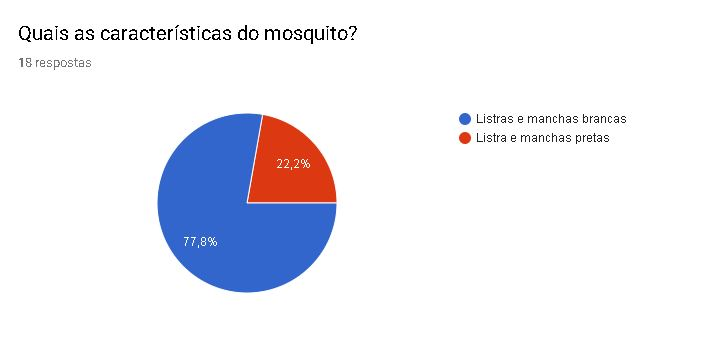
\includegraphics[width=0.7\linewidth]{Figuras/Pergunta_1}
		
		\label{fig:pergunta1}
	\end{figure}
	
	\begin{figure}[H]
		\centering
		\caption{Tivemos 88,9 \% de acertos}
		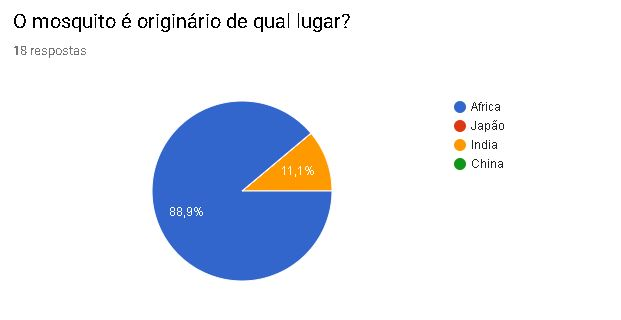
\includegraphics[width=0.7\linewidth]{Figuras/Pergunta_2}
		
		\label{fig:pergunta2}
	\end{figure}
	
	\begin{figure}[H]
		\centering
		\caption{Tivemos 88,9 \% de acertos}
		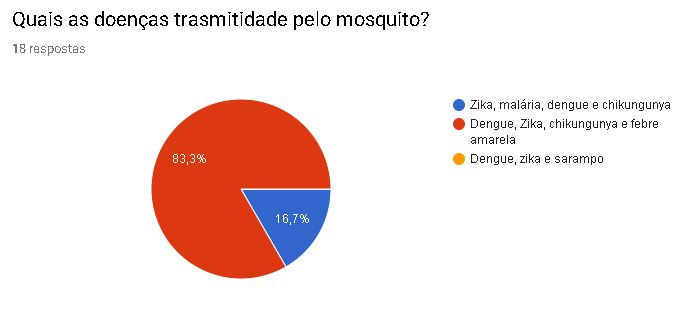
\includegraphics[width=0.7\linewidth]{Figuras/Pergunta_3}
		
		\label{fig:pergunta3}
	\end{figure}
	
	\begin{figure}[H]
		\centering
		\caption{Tivemos 88,9 \% de acertos}
		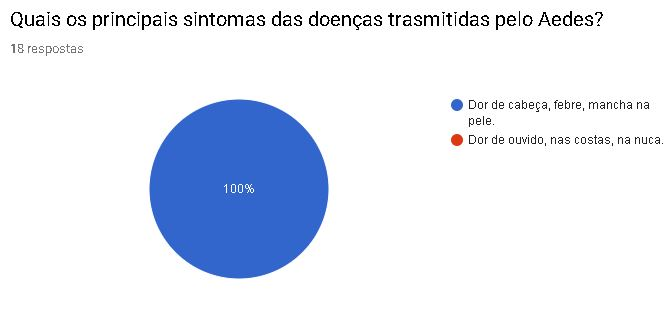
\includegraphics[width=0.7\linewidth]{Figuras/Pergunta_4}
		
		\label{fig:pergunta4}
	\end{figure}
	
	\begin{figure}[H]
		\centering
		\caption{Tivemos 88,9 \% de acertos}
		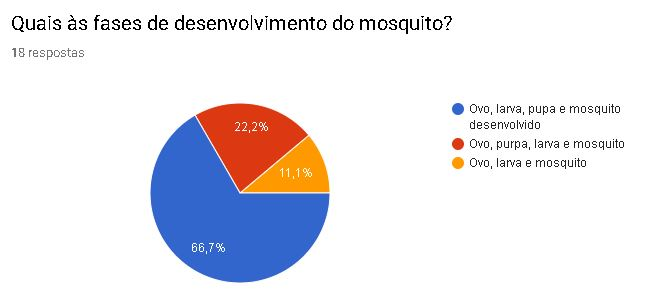
\includegraphics[width=0.7\linewidth]{Figuras/Pergunta_5}
		
		\label{fig:pergunta5}
	\end{figure}
	
	\section{Referências} 
	
	Links:\\ 	(Artigo sobre uso de jogos no ensino de programação)http://www.br-ie.org/pub/index.php/sbie/article/view/3000/2511\\
			(Pesquisa aplicada)https://galoa.com.br/blog/pesquisa-basica-e-pesquisa-aplicada-o-que-sao-e-suas-importancias\\
			(Evolução do ensino)http://www2.seduc.mt.gov.br/-/evolucao-historica-do-processo-ensino-aprendizag-3
	
	
	
\end{document}

